\section{Introduzione}
    I Ensembler sono algoritmi che costruiscono un insieme di classificatori di base ($\textbf{Weak Learners}$) e li utilizzano per classificare nuovi dati sulla base di un voto (pesato) delle loro previsioni.
    I metodi di ensemble di solito producono soluzioni più accurate rispetto a un singolo modello.
    \\[1\baselineskip]
    L'obiettivo degli Ensembler è combinare le previsioni di diversi stimatori di base costruiti con un dato algoritmo di apprendimento (es: Decision Trees) al fine di migliorare la generalizzabilità/robustezza su un singolo stimatore.
    \\[1\baselineskip]
    Generalmente si distinguono due famiglie di Ensemble Methods:

    \begin{itemize}
        \item $\textbf{Averaging Methods}\ (\textrm{o anche}\ \textbf{Bagging Methods}):$ l'obiettivo principale è costruire diversi stimatori in modo indipendente e quindi calcolare la media delle loro previsioni. In media, lo stimatore combinato è generalmente migliore di qualsiasi stimatore di base perché la sua varianza è ridotta;
        \\[1\baselineskip]
        \item $\textbf{Boosting Methods}:$ stimatori di base vengono costruiti in sequenza e si cerca di ridurre il bias dello stimatore di base successivo, aggiustando i pesi (sulla base dell'errore/precisione) per ogni campione di training in modo che gli stimatori successivi si possano concentrare su istanze erroneamente predette da quelli precedenti.
    \end{itemize}

    \begin{figure}[h]
        \caption[short]{Esempio di Bagging e Boosting}
        \centering
        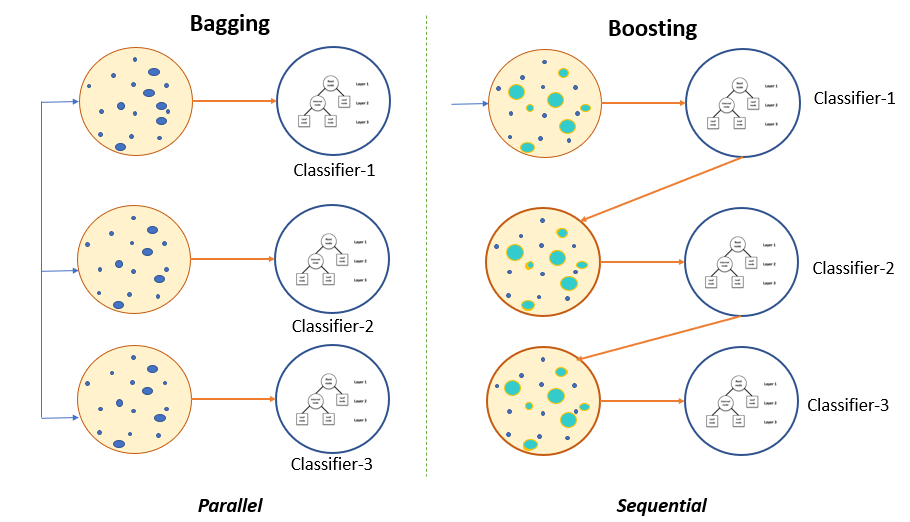
\includegraphics[width = 10cm, height = 7cm]{bagging-boosting-example.png}
    \end{figure}

    \clearpage